%% AMS-LaTeX Created with the Wolfram Language for Students - Personal Use Only : www.wolfram.com

\documentclass{article}
\usepackage{amsmath, amssymb, graphics, setspace}

\newcommand{\mathsym}[1]{{}}
\newcommand{\unicode}[1]{{}}

\newcounter{mathematicapage}
\begin{document}

\title{Wolfram Language and \(LATEX\)...}
\author{}
\date{}
\maketitle

\begin{doublespace}
\noindent\(\pmb{\text{mat} = \text{MatrixForm}[\text{Table}[\text{Sin}[j x{}^{\wedge}i +i y{}^{\wedge}j],\{j,1,5\},\{i,1,5\}]];}\\
\pmb{\text{Print}[\text{mat}];}\)
\end{doublespace}

\noindent\(\left(
\begin{array}{ccccc}
 \text{Sin}[x+y] & \text{Sin}\left[x^2+2 y\right] & \text{Sin}\left[x^3+3 y\right] & \text{Sin}\left[x^4+4 y\right] & \text{Sin}\left[x^5+5 y\right]
\\
 \text{Sin}\left[2 x+y^2\right] & \text{Sin}\left[2 x^2+2 y^2\right] & \text{Sin}\left[2 x^3+3 y^2\right] & \text{Sin}\left[2 x^4+4 y^2\right] &
\text{Sin}\left[2 x^5+5 y^2\right] \\
 \text{Sin}\left[3 x+y^3\right] & \text{Sin}\left[3 x^2+2 y^3\right] & \text{Sin}\left[3 x^3+3 y^3\right] & \text{Sin}\left[3 x^4+4 y^3\right] &
\text{Sin}\left[3 x^5+5 y^3\right] \\
 \text{Sin}\left[4 x+y^4\right] & \text{Sin}\left[4 x^2+2 y^4\right] & \text{Sin}\left[4 x^3+3 y^4\right] & \text{Sin}\left[4 x^4+4 y^4\right] &
\text{Sin}\left[4 x^5+5 y^4\right] \\
 \text{Sin}\left[5 x+y^5\right] & \text{Sin}\left[5 x^2+2 y^5\right] & \text{Sin}\left[5 x^3+3 y^5\right] & \text{Sin}\left[5 x^4+4 y^5\right] &
\text{Sin}\left[5 x^5+5 y^5\right] \\
\end{array}
\right)\)

\begin{doublespace}
\noindent\(\pmb{\text{}}\\
\pmb{\text{Clear}[x,y,z]}\\
\pmb{\text{picture} = \text{Show}[}\\
\pmb{\text{ContourPlot3D}[\{z==x y,x+y==1,z==0\},\{x,-1,2\},\{y,-1,2\},\{z,-1,2\}],\text{RegionPlot3D}[z\text{$<$=} x y\&\&x+y\leq  1\&\&x\geq 0\&\&y\geq
0\&\&z\geq  0,}\\
\pmb{\{x,-1,2\},\{y,-1,2\},\{z,-1,2\},\text{PlotPoints}\to 50]}\\
\pmb{]}\)
\end{doublespace}

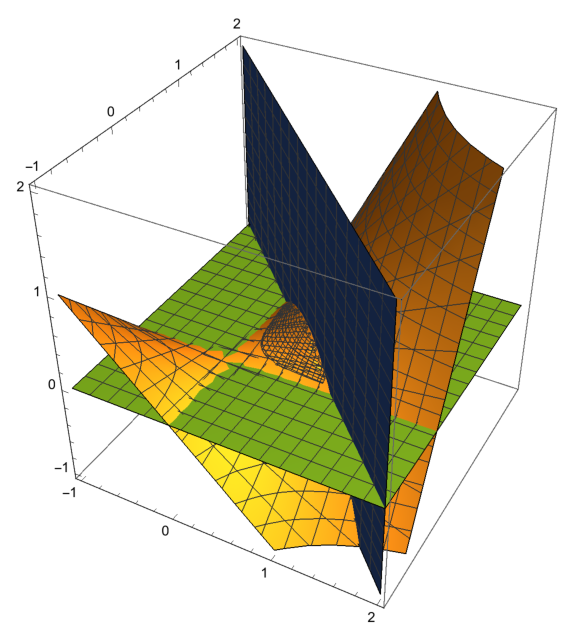
\includegraphics{wf-tex-pdf_gr1.eps}

\end{document}
